\setcounter{NAT@ctr}{-1}
\chapter*{}
\phantomsection\addcontentsline{toc}{section}{Galactic Circos}

\begin{figure}[t!]
\centering

\includegraphics[height=10em]{frontmatter/images/chapter-header-circos.png}
\end{figure}
\vspace{-4cm}


\articletitle{Galactic Circos: User-friendly creation of Circos Plots within the Galaxy platform}

Helena Rasche \textsuperscript{\ref{affil:freiburg},*},
Saskia Hiltemann\textsuperscript{\ref{affil:emc-bioinf},*}

{\color{chaptergrey}{*}} Helena Rasche and Saskia Hiltemann contributed equally to this work.

\textbf{Published in:} \emph{GigaScience}, Volume 9, Issue 6, June 2020, giaa065 \\
\textbf{DOI:} \url{https://doi.org/10.1093/gigascience/giaa065}

\small
\begin{enumerate}
 \itemsep-0.5em
 \item Bioinformatics Group, Department of Computer Science, University of Freiburg, 79110 Freiburg im Breisgau, Germany\label{affil:freiburg}
 \item Erasmus Medical Center, Clinical Bioinformatics Group, Department of Pathology, Rotterdam, The Netherlands.\label{affil:emc-bioinf}
\end{enumerate}



\section*{Abstract}

\textbf{Background:} Circos is a popular software package for circular visualisation of complex datasets. Circos is a highly flexible tool and is especially popular in the field of genomics, though it may be applied to any type of data. This high degree of flexibility also comes with a high degree of complexity, which may present an obstacle for researchers not trained in programming or the UNIX command line. Galaxy provides a user-friendly web interface for such commandline tools, greatly improving their accessibility.
% - no way to generate pub quality plots in Galaxy
% - circos fills this space for bioinformaticians
% - but it's incredibly complex

\textbf{Findings:} We have developed a Galaxy wrapper for Circos, thus combining the power of Circos with the accessibility and ease-of-use of the Galaxy platform. This significantly simplifies the specification of Circos plots for end-users while retaining the power to produce publication-quality visualization of multidimensional complex datasets.

% - built a galaxy tool wrapper for circos
% - it provides user-friendly interface to the vast array of circos options
%- it leverages galaxy's existing templating to build circos config

\textbf{Conclusions:} Galactic Circos enables the creation of publication-ready Circos plots within the Galaxy platform. Users may download the full configuration of their plots for further manual tweaking. This tool has been made available from the Galaxy Tool Shed (\url{https://toolshed.g2.bx.psu.edu/view/iuc/circos}), and is accompanied by a Galaxy training manual (\url{https://training.galaxyproject.org}).
%- easy pub-quality plots
%- users can download plots and continue editing them

\textbf{Keywords: } Genomics; Visualisation; Galaxy; Circos; UI/UX


\section*{Findings}

\subsection*{Background}

%\begin{epigraph}{Circo's Author, M. Krzywinski}
%The biological scientific community has adopted Circos wholeheartedly. By now, Circos has appeared on the the covers of both Nature and Science publications, which are the world's top scientific journals.
%\end{epigraph}

% intro to Circos and its shortcomings (user-friendliness)
The Circos visualization tool \cite{krzywinski2009} is widely used in the biological scientific community, and is especially popular for use in scientific publications. Circos has over 4000 citations, and its plots have appeared on the cover of several leading scientific journals \cite{circospubs}. Its popularity is due in a large part to its great flexibility; Circos offers a wide range of visualisation options, and all aspects of a Circos plot may be tweaked and customized to the user's wishes. While originally created for the visualisation of genomic data, Circos makes no a priori assumptions about the format and domain of the input data; this is illustrated by the fact that it has been used for a wide range of applications, ranging from genomics research to visualisations of car sales, urban planning, and even presidential debates \cite{circosnongenomic}.

With Circos's great flexibility also comes a high degree of complexity, and a significant learning curve, and as a result its use is often limited to expert users who are experienced with programming and the UNIX command line.

% intro to Galaxy and how it complements Circos in terms of providing the user-friendliness it lacks
The Galaxy platform \cite{afgan2018galaxy} aims to provide a user-friendly interface to commandline tools, and empower domain experts to run powerful analysis and visualization tools without the need for any programming experience. Galaxy offers a wide range of tools for a variety of applications domains, and is widely used in the biological scientific community (7000+ citations, 7200+ tools \cite{galaxycitations,galaxytoolshed}). Galaxy also automates the installation of tools and all their dependencies, removing another hurdle for its use by research scientists.

% sentence about galactic circos combining best of both worlds and being awesome
Our tool combines the power of Circos with the user-friendliness of the Galaxy interface to greatly increase the accessibility of the tool and simplify the creation of publication-ready plots for scientific data.

Previously, custom Circos Galaxy plotter tools have been written \cite{hiltemann2014cgtag}; however, these tools are not generic, but are tailored specifically to the use case at hand. This means that a new Galaxy tool has to be created whenever a new plot type is needed. Galactic Circos aims to be a generic tool capable of creating any Circos plot regardless of data domain.

\subsection*{Results}
The Galactic Circos tool changes the way users must specify the configuration of a Circos plot. Instead of writing a number of configuration files, users now only need to select the various plot options from a web interface (Figure \ref{figure:userinterface}). Because Circos plot specifications can be quite complex, the tool interface is subdivided into several collapsible sections, each corresponding to a different Circos configuration option in order to increase the usability of the tool. Parameters are preconfigured with sensible default values so that basic plots can be generated with minimal configuration.

\begin{figure}[h!]
\centering
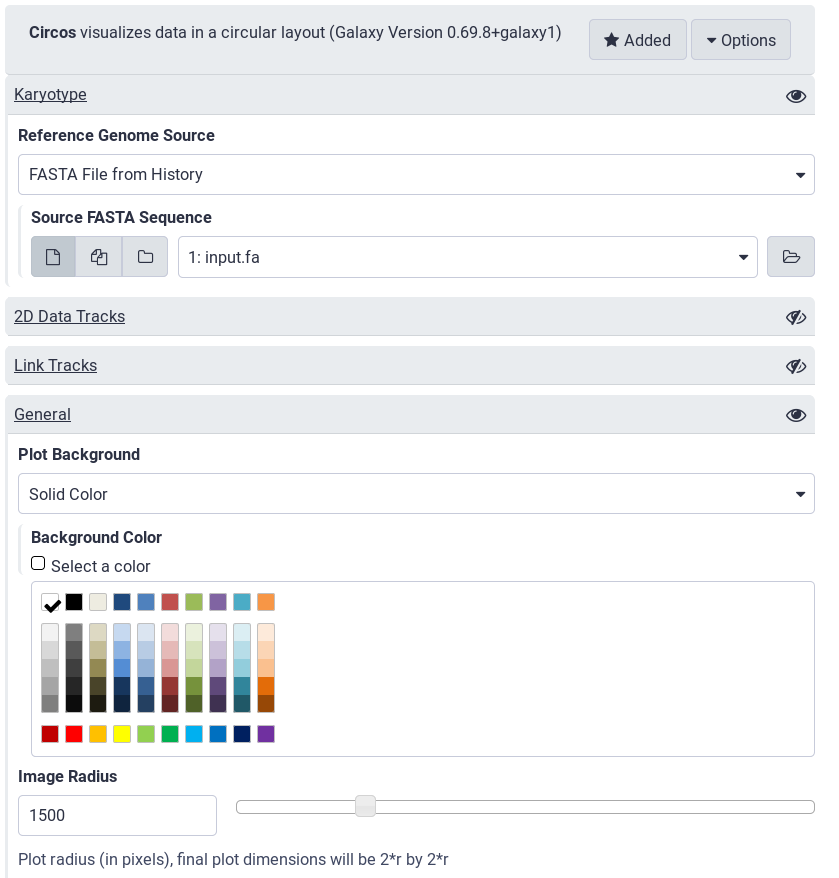
\includegraphics[width=0.8\linewidth]{chapters/images/circos/circos-galaxy-ui.png}
\caption{The Galaxy tool interface to Circos. Each collapsed section hides a wealth of configuration options available to users. The web based interface is significantly more accessible than the command line version.}\label{figure:userinterface}
\end{figure}

We demonstrate the utility of the Galactic Circos tool by recreating one of the more advanced examples from the Circos online tutorials, the microbial genome lesson \cite{circos-microbial-example} (Figure \ref{figure:microbe}). This displays multiple tracks of different types (text, histogram, tiles), has a customized ideogram, and uses rules for colouring data points dependent on their value.

\begin{figure}[h!]
\centering
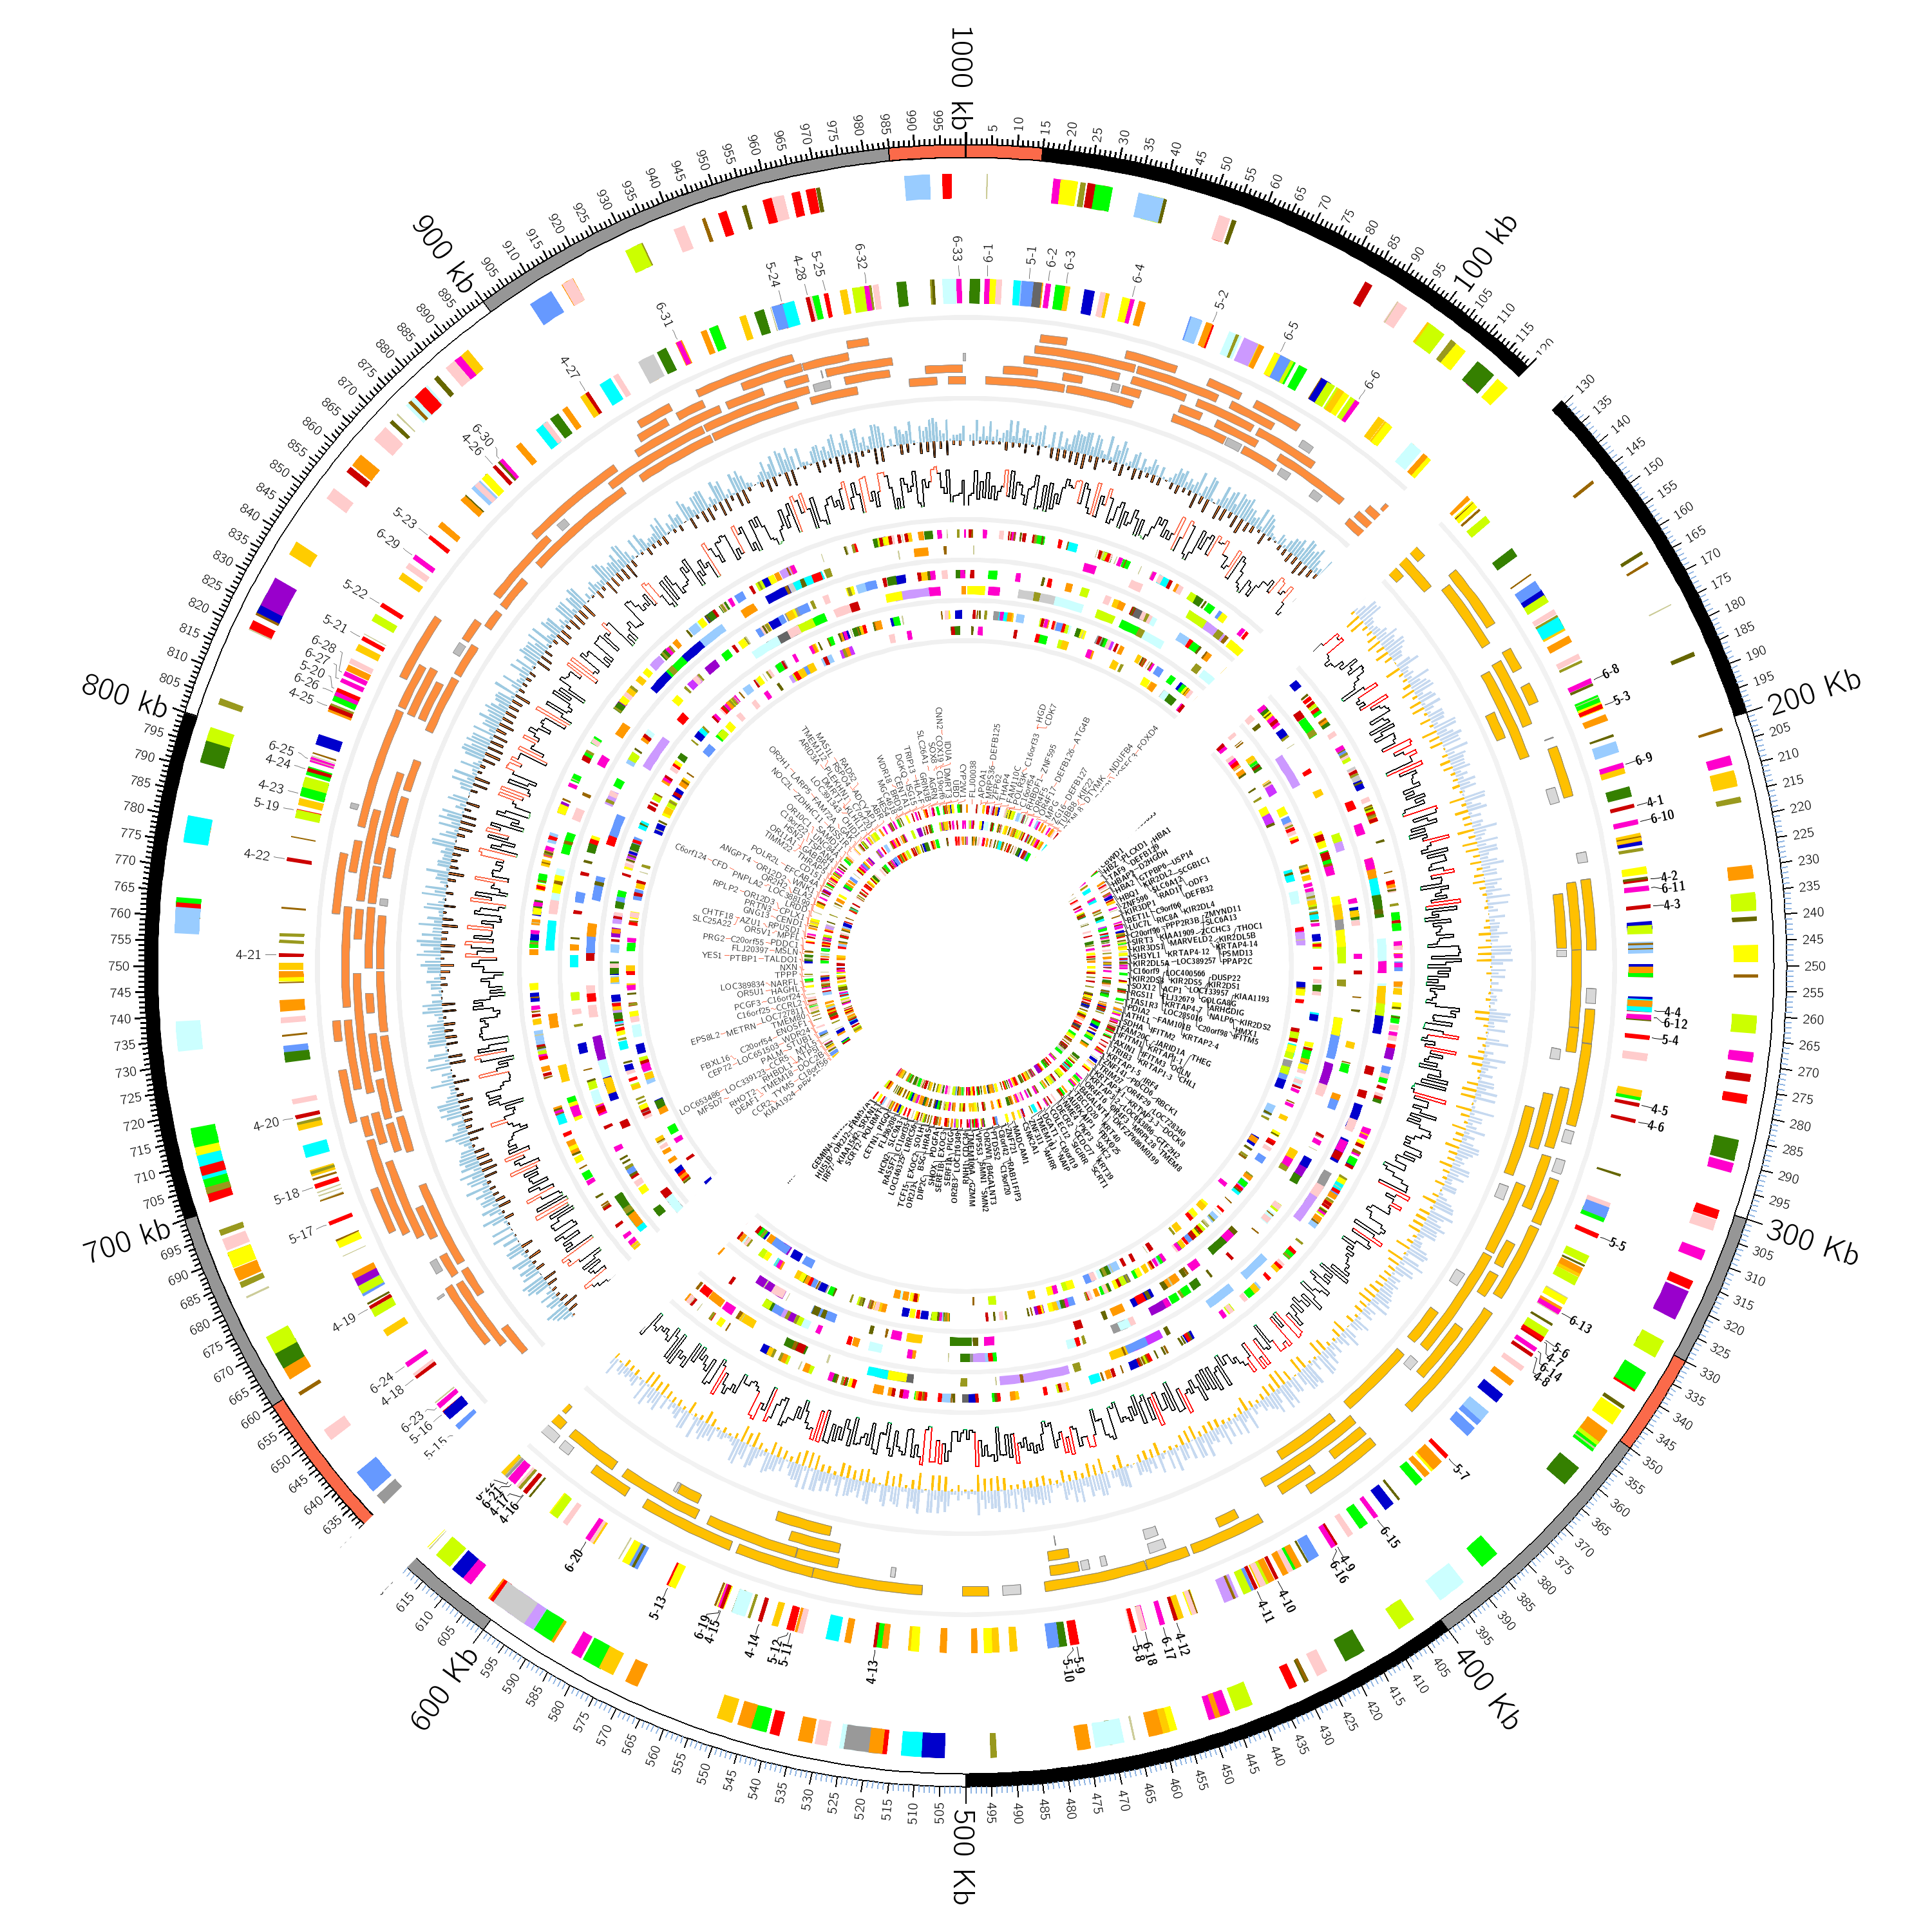
\includegraphics[width=0.8\linewidth]{chapters/images/circos/plot-microbe-both.png}
	\caption{Here we reproduce one of the more complex tutorials from the Circos documentation. The top-left half of the image is produced by the configuration provided by the Circos tutorial, while the bottom-right half is produced completely in Galaxy. While some options used in the original tutorial cannot be directly used (e.g. unrestricted perl code), they can be recreated equivalently in the tool interface. Some options in the tool interface are likewise restricted, Galactic Circos offers a color picker with a limited palette, which explains the differences in colour. However, our tool offers the ability to download the full Circos configuration folder, allowing advanced users to tweak the colour (or other) parameters manually and rebuild the image locally.}\label{figure:microbe}
\end{figure}

In a second example (Figure \ref{figure:encode}), we replicate within Galaxy the cover image of the Nature issue \cite{nature-encode} dedicated to the ENCODE project \cite{encode2004encode}. This cover featured a Circos plot and is also available as part of the official Circos tutorials \cite{circos-nature-example}.

\begin{figure}[h!]
\centering

\includegraphics[width=0.7\linewidth]{chapters/images/circos/plot-encode-both.png}
\caption{Nature's cover for the ENCODE project in September 2012, reproduced by Galactic Circos. The top-left half of the image is again directly from the cover, whilst the bottom-right half shows the reproduction of the image using the Galactic Circos tool. The full image could be reproduced in Galaxy accurately, if one wished.}
\label{figure:encode}
\end{figure}

These two examples showcase a variety of different track types (histograms, scatterplot, highlights, tiles, text) and configurations (ticks, rules, ideogram customizations) to illustrate the feature-completeness of Galactic Circos. % "What features" -A

\subsubsection{Supporting Tools}
Circos requires input datasets to adhere to a specific and custom file format. In order to facilitate the conversion of data to this custom Circos format, we have developed several supporting Galaxy tools for conversion. These tools allow users to convert their datasets from a variety of common genomics formats such as (big)Wig files, interval files, and MAF alignments. Furthermore, the existing Galaxy ecosystem provides a wide array of tabular data manipulation tools that can be leveraged to transform any tabular or text files into the format accepted by Circos.

To demonstrate the utility of these supporting tools, we show a real-world example of a plot using common genomics datasets. This example is a recreation of a plot in a published paper demonstrating chromothripsis in the VCaP prostate cancer cell line \cite{alves2013gene}. The input datasets originate from a variety of sources, including a structural variants files (converted to Circos links track), copy number and B-allele frequency track obtained from Affymetrix SNP array data, and a SNP density track generated from a VCF file. Using a combination of the supporting tools included in the Galactic Circos package and the generic file manipulation tools present in Galaxy, we were able to convert these various datasets to circos format without leaving Galaxy, and reproduced the Circos plot from the publication (Figure \ref{figure:vcap}).

\begin{figure}[h!]
\centering
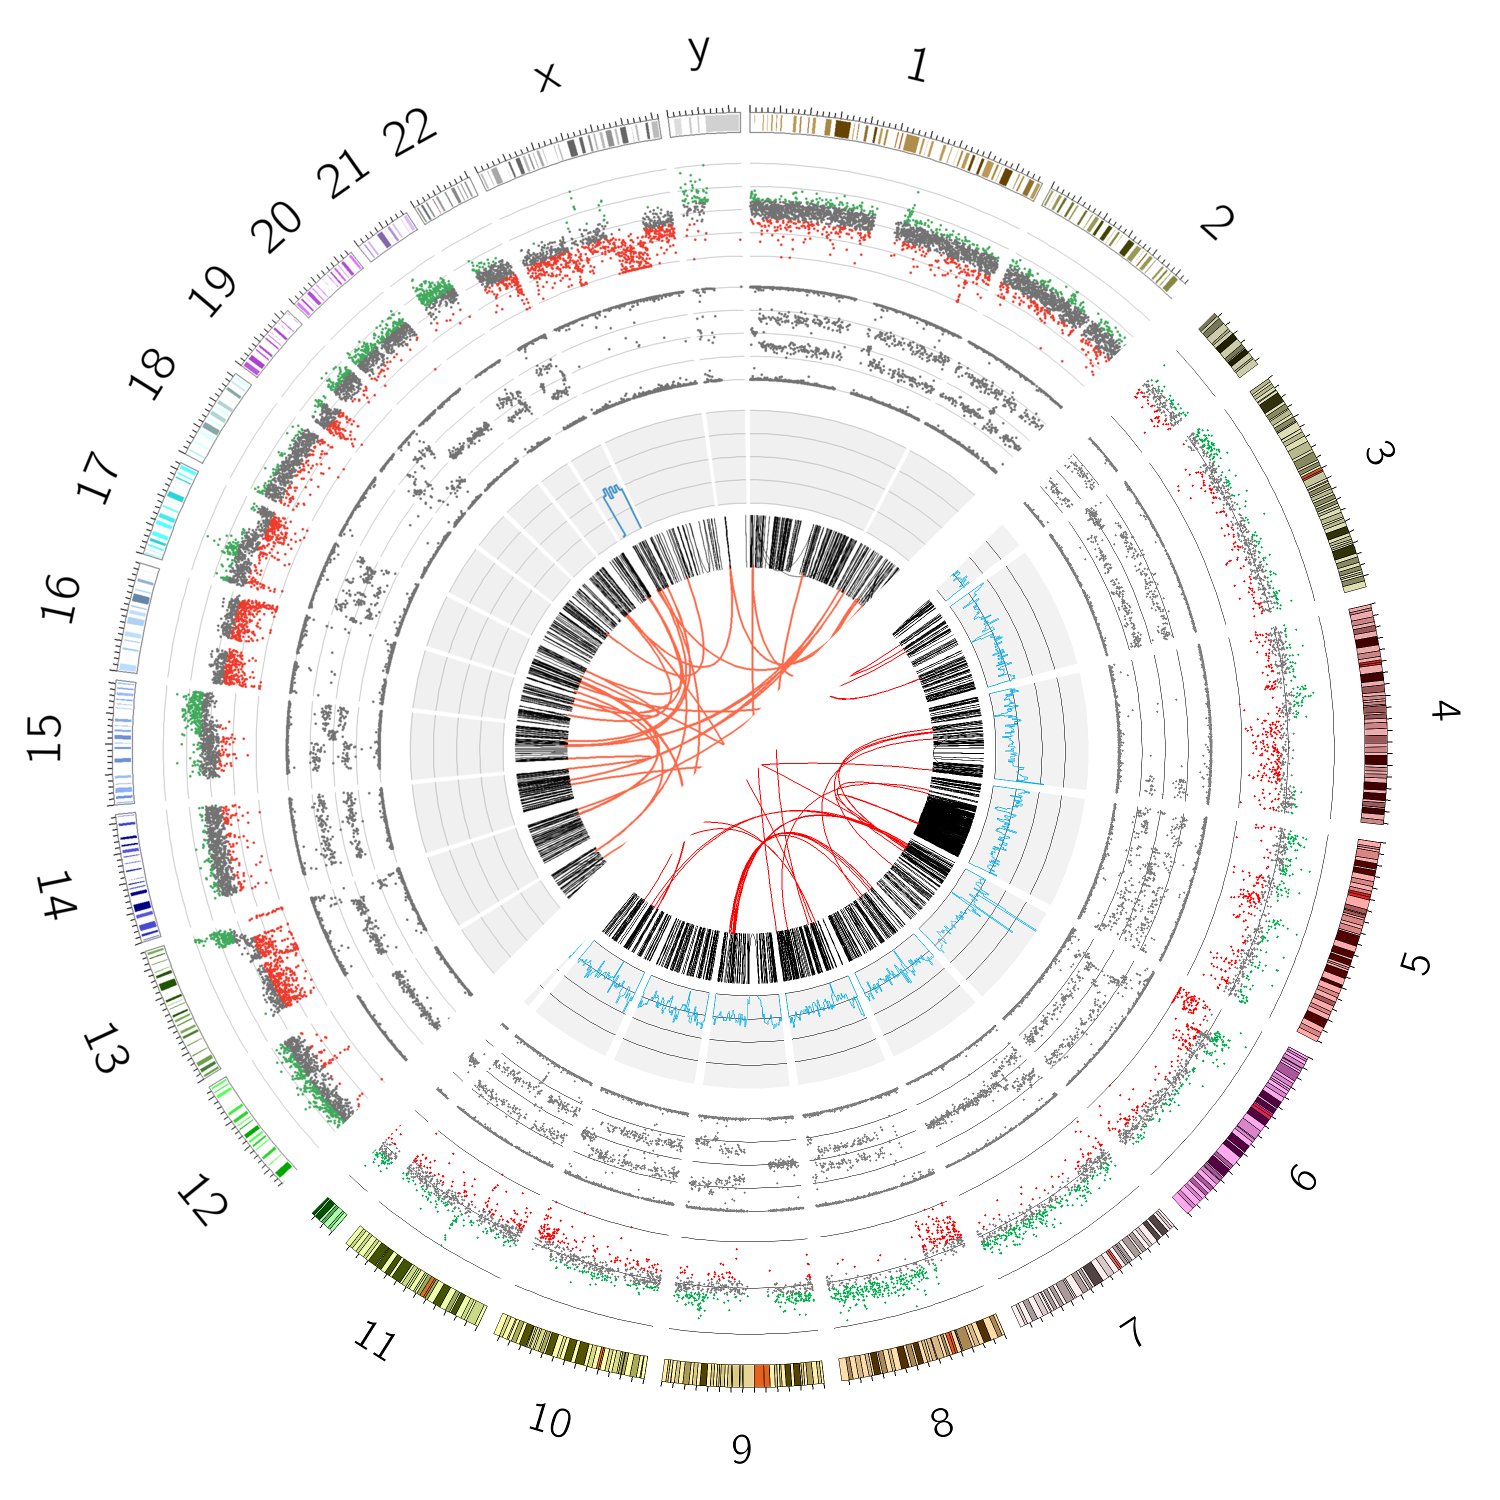
\includegraphics[width=0.6\linewidth]{chapters/images/circos/plot-complete-genomics-both.png}
	\caption{This figure compares output of a custom written Circos plot with hardcoded configuration (top left half), to ťhe output created using the Galactic Circos tool (bottom right half). While the input data originated from a range of standard and nonstandard genomic file formats, conversion to circos-formatted files was possible using the plethora of file manipulation tools already integrated into Galaxy and the set of supporting conversion tools included in the Galactic Circos package.}
\label{figure:vcap}
\end{figure}

Once data has been reformatted for Circos, it can either be used immediately or be further processed. Circos includes a tool suite for post-processing and downsampling of data which can improve plot clarity and processing speed. We additionally wrapped a number of these post-processing tools into Galaxy, notably the link bundling and binning scripts seen in Figure \ref{figure:binning-bundling}.

\begin{figure}[h!]
\centering
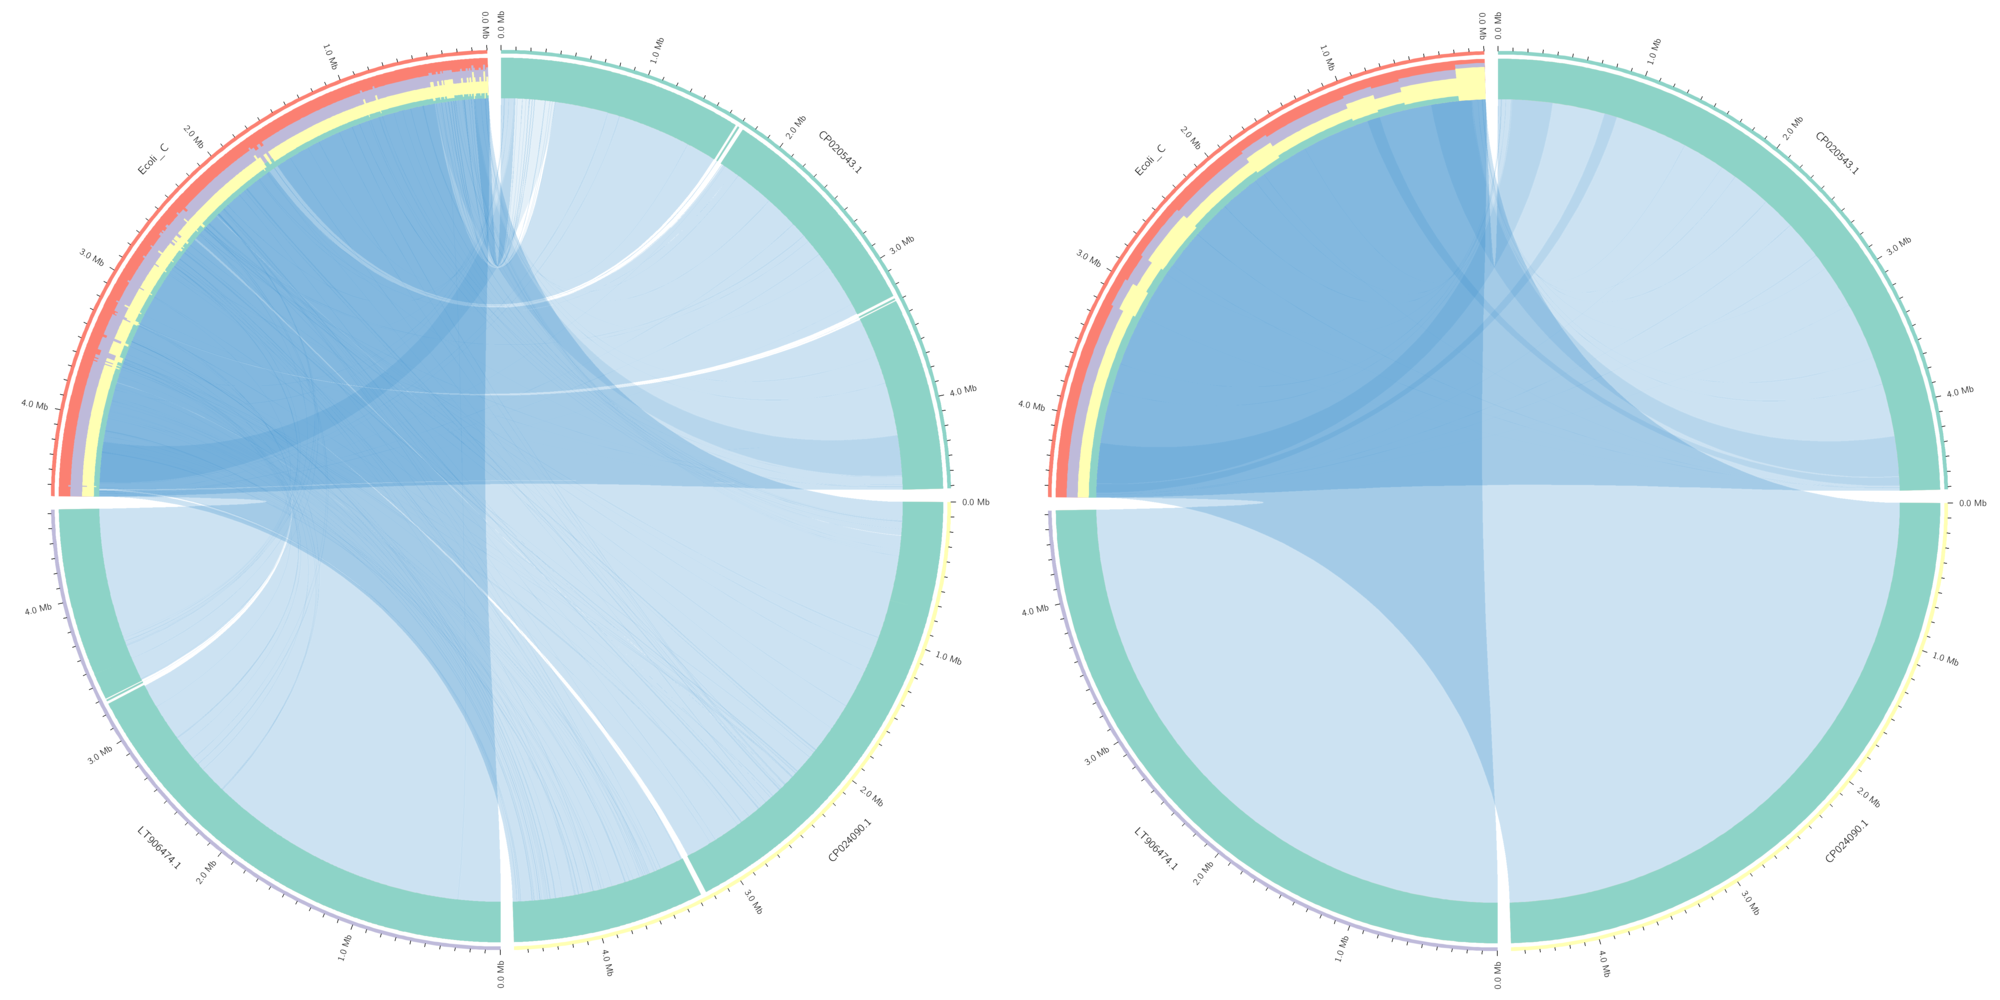
\includegraphics[width=\linewidth]{chapters/images/circos/binning-bundling.png}
\caption{These two plots show the link binning and bundling scripts used with different thresholds. The inner link track was generated directly from a MAF file output by LastZ \cite{rahmani2011lastz}. This file was processed by Circos' bundling tool in Galaxy in order to decrease the number of links, a process usually done to decrease visual noise and increase efficiency. The outer track demonstrates the link binning script which generates a histogram, in this case from the number of links to that position in the genomic region.}
\label{figure:binning-bundling}
\end{figure}

Finally, while Circos is widely used for the visualization of genomic data, and many of the parameter names have a distinctly biological feel to them, the tool does not impose any restrictions on the type of input data, and is capable of displaying non-biological data just as easily \cite{circosnongenomic}. To show that our tool retains this degree of flexibily, we recreated the presidential debate plot included in the Circos tutorials, which in turn was based on a plot which appeared in the New York Times aticle \cite{namingnames}. A plot comparison can be seen in Figure \ref{figure:debate}.

\begin{figure}[h!]
\centering
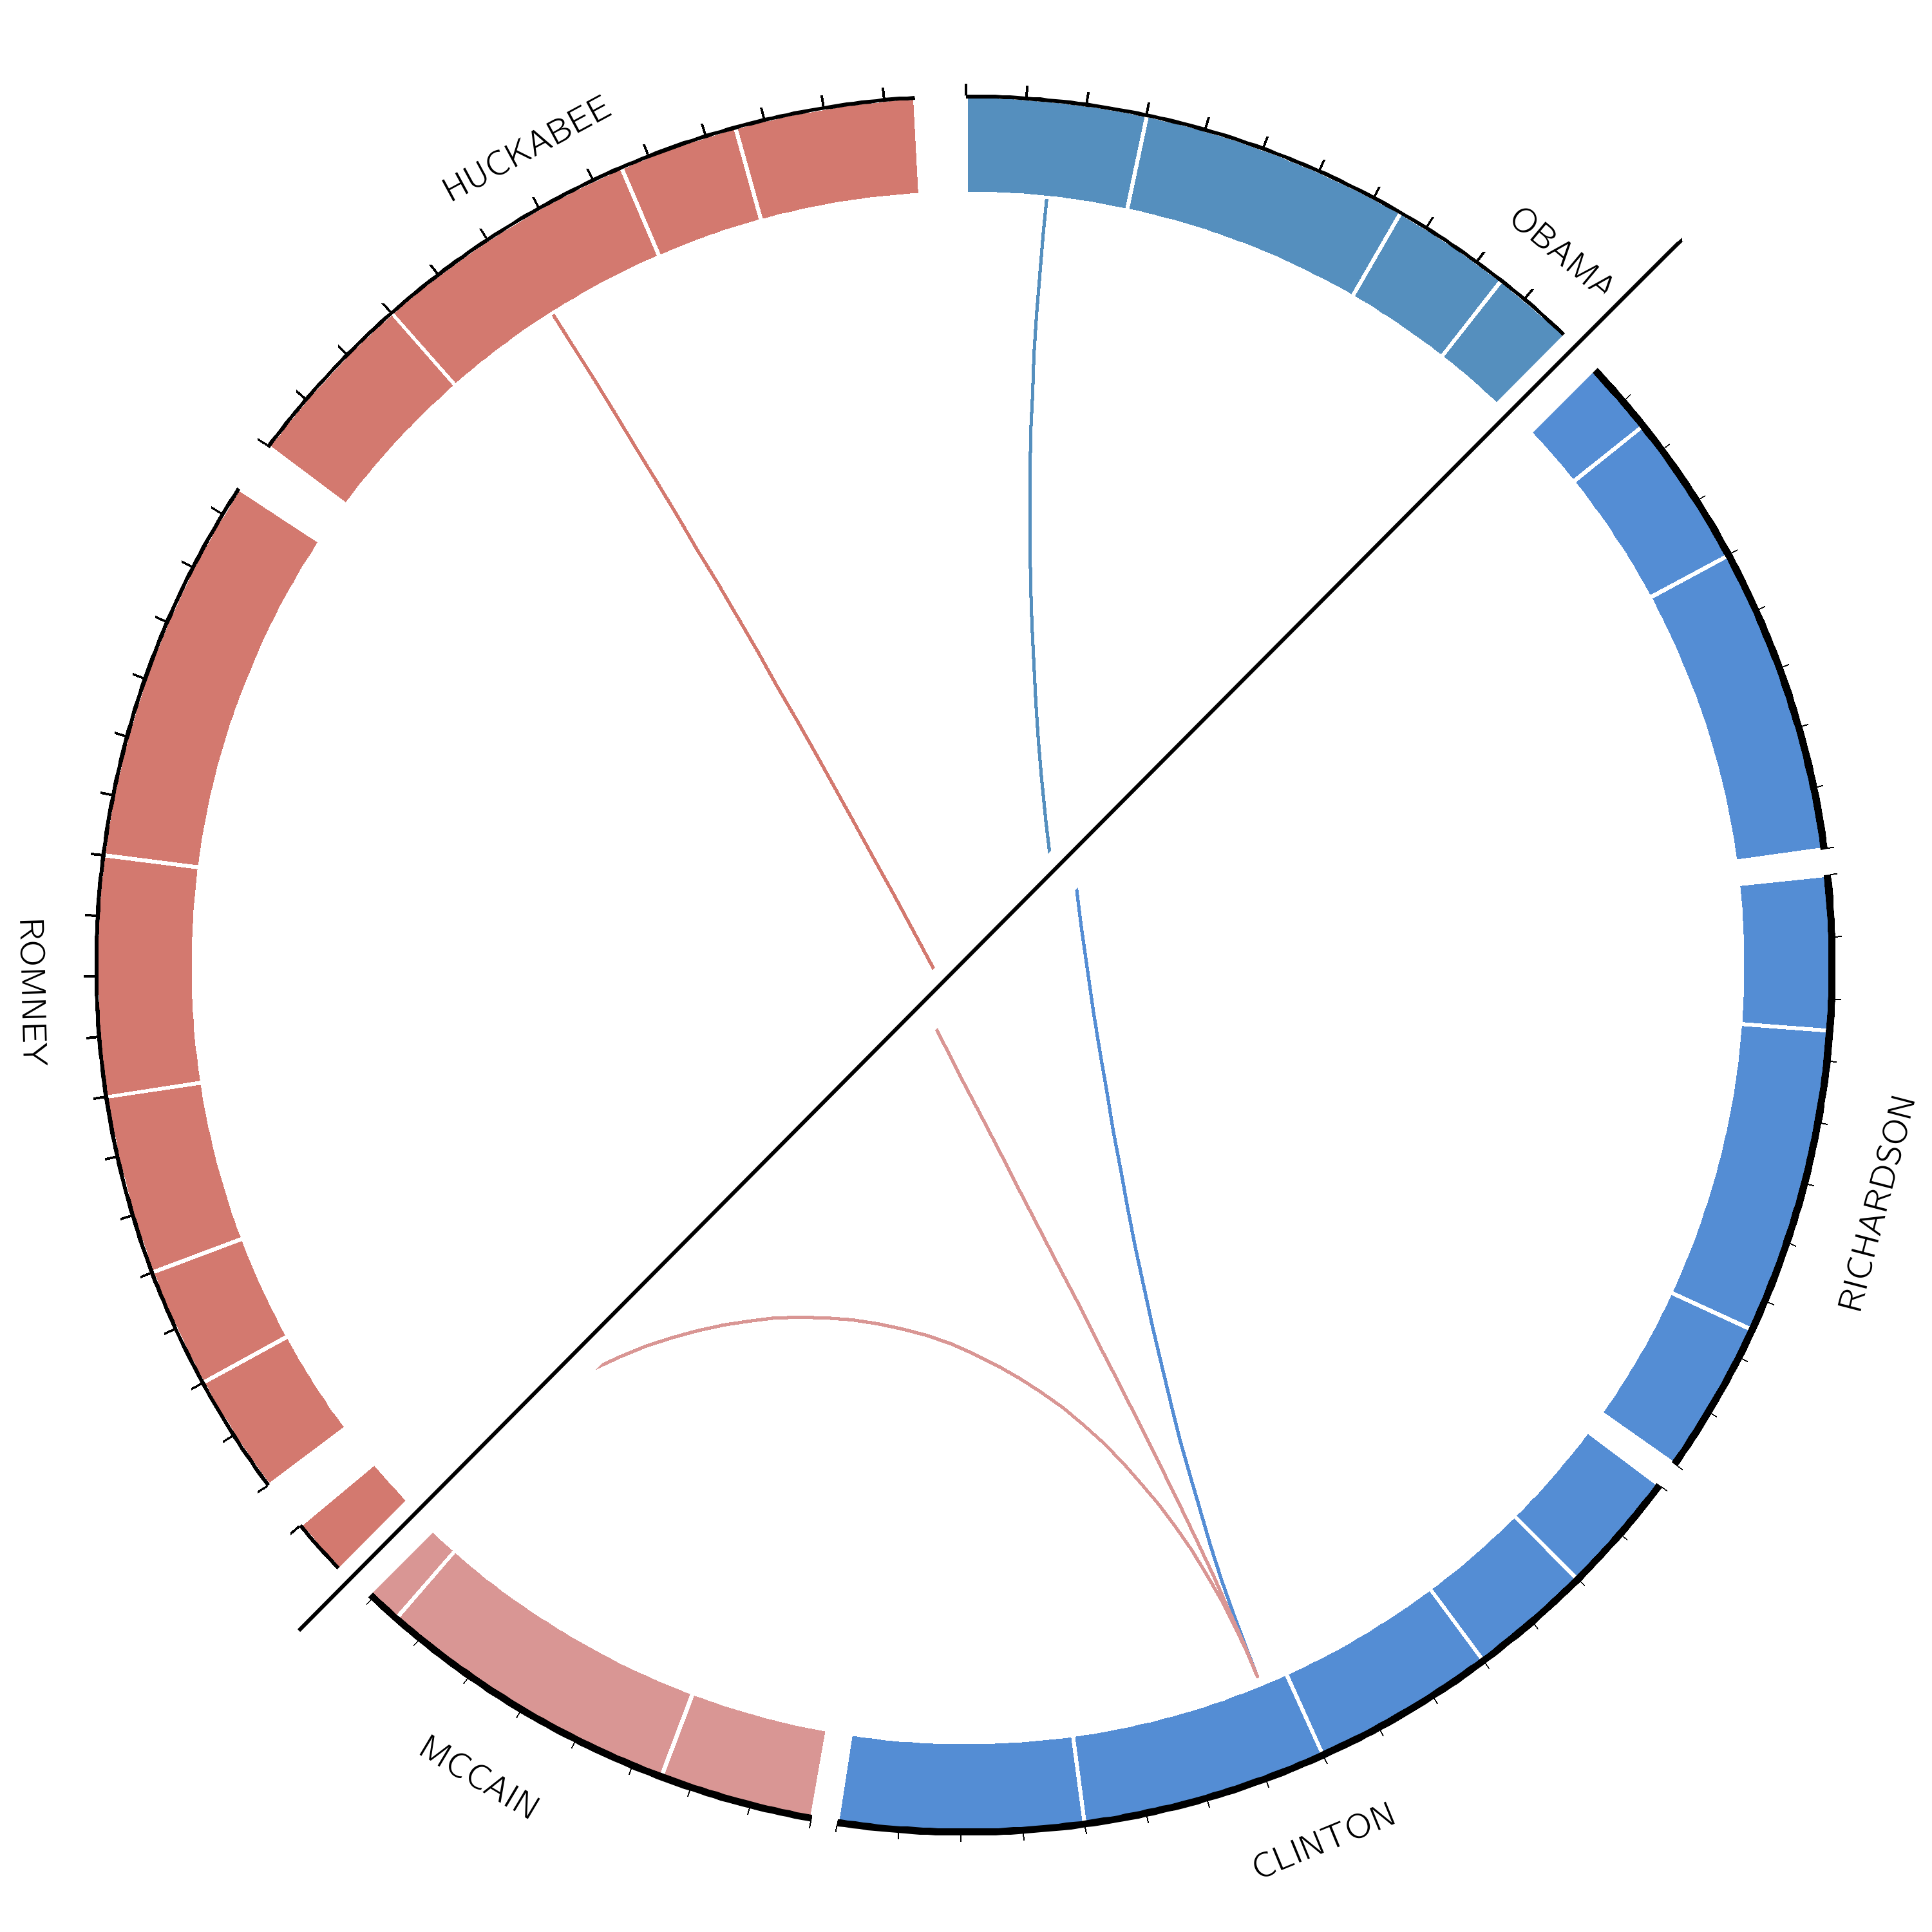
\includegraphics[width=0.6\linewidth]{chapters/images/circos/plot-politics-both.png}
\caption{This figure compares the Circos plot from the official tutorial (top left half), to ťhe output created using the Galactic Circos tool (bottom right half). Each link represents a candidate speaking the last name of another candidate. The length of each circle segment is proportional to the total number of words spoken by the candidate during the debates.}
\label{figure:debate}
\end{figure}

\section*{Methods}

\subsection*{Implementation}
The execution of the tool leverages Galaxy's ability to write templated files directly to disk with configuration from the tool form, and then running Circos directly on these templated configuration files.

Installation of the Circos tool and its dependencies is handled by the Galaxy platform and utilizes the Conda framework for dependency management. All dependencies including circos itself are available from the Bioconda Conda channel \cite{gruning2018bioconda} and available as a virtualised container (rkt, Docker, Singularity).

\subsection*{File Format Converters}
In order to facilitate the interoperability with upstream tools and workflows, we provide a set of file format converters, in addition to many tools already available in Galaxy, which together provide for convertion of a range of common data format standards (e.g. VCF, MAF/Stockholm, BED/GFF3, BigWig). These tools produce files that are ready to be used as input to the Galaxy Circos tool. Additionally the applicable subset of circos-utils were included into Galaxy for Circos-friendly tools for data reshaping.

\subsection*{Circos Configuration Export}
While Galactic Circos aims to offer the full range of Circos functionality, some manual tweaking of the Circos plot configuration files may still be desired. To this end, our tool also outputs the full set of configuration files needed to recreated the plot on the command line, and thus allow easy access to any features not exposed in the Galaxy wrapper.

\subsection*{Training Materials}
Our tool greatly simplifies the creation of Circos plots, but the great number of options offered by the Circos tool require good documentation and explanation in order to optimize their utility for end-users. Circos offers a collection of tutorials that are designed to familiarize users with the various features of Circos \cite{circostutorials}. In a similar fashion, we have created a set of Galaxy tutorials aimed to educate users in the use of Circos within Galaxy. These tutorials are available from the Galaxy training materials website \cite{Batut2018}.

\subsection*{Reproducible and Reusable Plots}
To enable readers to examine the complete parameters settings used and recreate the example plots given here, Galaxy histories for all the figures shown in this work have been made publicly available from the European Galaxy server \cite{TODO} (see Availability section).

\subsection*{Future Work}
While we have aimed to make our tool as feature-complete as possible, some of Circos' functionality is not currently exposed in the Galaxy tool. We intend to extend our tool to include these features, including but not limited to support for scaling subsections of the plots, and generation of HTML image maps.

\section*{Availability of source code and requirements}
\begin{itemize}
\item Project name: ~Galactic Circos
\item Github repository:~\url{https://github.com/galaxyproject/tools-iuc/tree/master/tools/circos}
\item Tool Shed repository: ~\url{ https://toolshed.g2.bx.psu.edu/view/iuc/circos}
\item Training Manual: ~\url{https://training.galaxyproject.org/<TODO>}
\item Operating system(s): ~Unix (~Platform independent with Docker)
\item Other requirements: ~Galaxy version 18.01 or higher
\item License: ~GNU GPL
\end{itemize}

The Circos example plots presented in this work are available as Galaxy histories:

\begin{itemize}
\item Galaxy history for Figure 2: https://usegalaxy.eu:/u/helena-rasche/h/circos-microbe-tutorial
\item Galaxy history for Figure 3: https://usegalaxy.eu/u/helena-rasche/h/circos-encode-nature-cover
\item Galaxy history for Figure 4: https://usegalaxy.eu/u/helena-rasche/h/circos-cancer-genomics--chromothripsis
\end{itemize}

\section*{Availability of supporting data and materials}

The data presented here to illustrate our application was obtained from previous publications, and has been collected and made available from Zenodo \cite{TODO}.

\section*{Declarations}

\subsection*{List of abbreviations}

\begin{itemize}
\item NGS: Next Generation Sequencing
\item VCF: Variant Call Format
\item MAF: Multiple Alignment Format
\end{itemize}

\subsection*{Competing Interests}
The authors declare that they have no competing interests.

\subsection*{Funding}
This project was made possible with the support of the Albert Ludwig University of Freiburg.

This project has received funding from the European Union’s Horizon 2020 research and innovation programme under grant agreement 825775.

\subsection*{Author's Contributions}

HR and SH contributed to the tool development and writing of the manuscript.

\section*{Acknowledgements}

The authors would like to thank the Galaxy community for their help in reviewing, testing, and validating the tools presented here.

\bibliographystyle{ieeetr}
\bibliography{references}
